\section{Decay-time acceptance}
\label{sec:Acceptance}

The decay-time distribution of the $\Bs$ mesons is distorted due to the geometry of the LHCb detector and the applied selections, described in Section \ref{sec:Selection}.
In particular, any requirement on the flight distance, the impact parameter or the direction angle (DIRA) of the $\Bs$ mesons leads to a decay-time dependent efficiency $\epsilon(t)$.
This acceptance effect in the $\Bs\to\Ds\kaon\pion\pion$ decay-time distribution is strongly correlated wih the CP parameters. \newline
However, for the flavour-specific control channel $\Bs\to\Ds\pion\pion\pion$, the acceptance can be measured since all CP-violating parameters are fixed to zero or unity. 
Using $\Gs$ as input, the parameters of the acceptance shape, as well as $\dms$, is measured using a time-dependent fit to the background-subtracted decay-time distribution of $\Bs\to\Ds\pion\pion\pion$ candidates.
To correct small differences between the signal and the control sample, 
the fit is performed simultaneously to the decay-time distributions of simulated  $\Bs\to\Ds\pion\pion\pion$, $\Bs\to\Ds\kaon\pion\pion$, as well as to $\Bz\to\Ds\kaon\pion\pion$ data candidates.
For all samples, the acceptance is parametrized using segments of cubic b-splines, which are implemented into the decay-time PDF in an analytic way~\cite{Karbach:2014qba}.
The decay-time distribution of background-subtracted $\Bs\to\Ds\pion\pion\pion$ data candidates, as well as the time-dependent fit to determine the accpetance shape, is shown in Figure~\ref{fig:accFit}.

\begin{figure}[h]
\centering
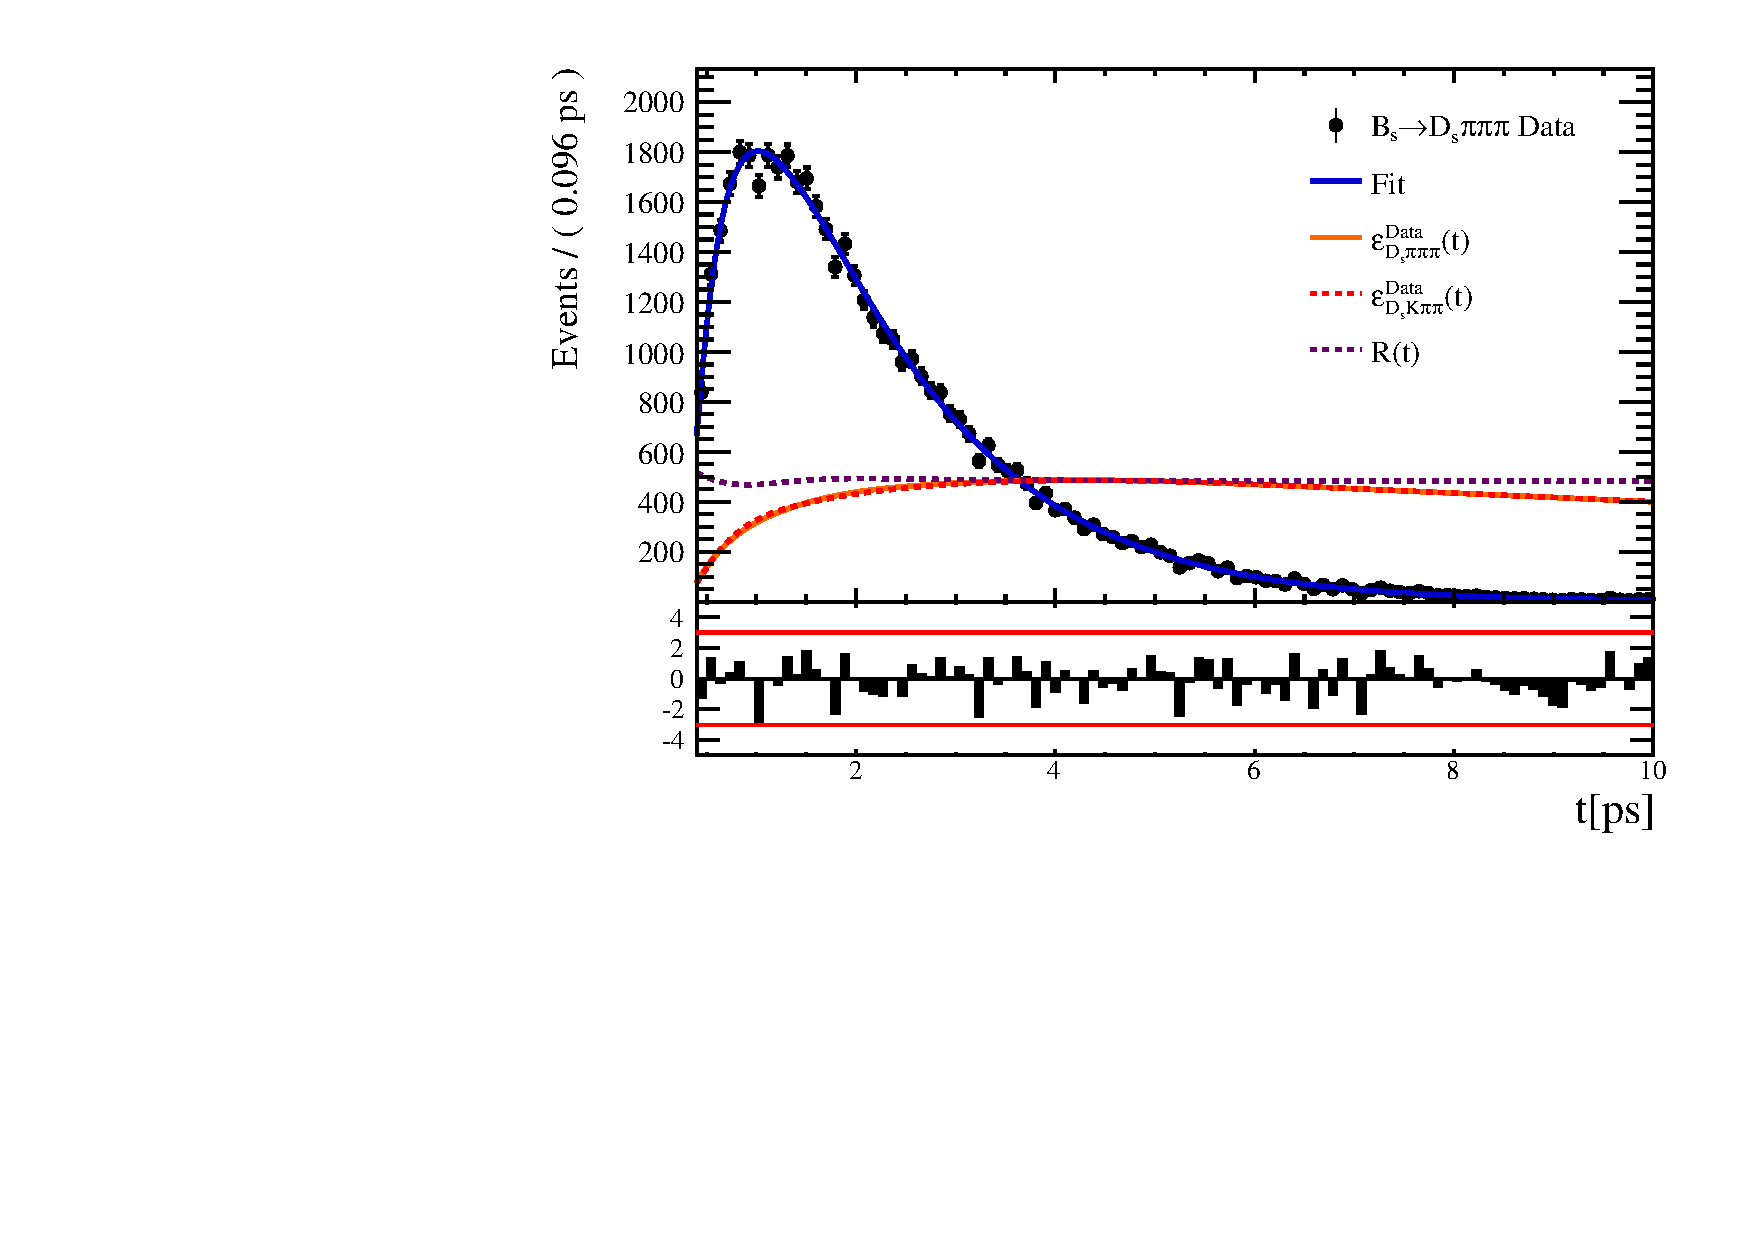
\includegraphics[height=!,width=0.65\textwidth]{figs/Acceptance/adaptive_N4/timeAccRatioFit_norm_Run2_t0.pdf}
\caption{Decay-time distribution of background-subtracted $\Bs\to\Ds\pion\pion\pion$ data. The fit to determine the shape of the time-dependent efficiency is overlaid, where the acceptance function is shown in an arbitrary scale.}
\label{fig:accFit}
\end{figure}

